%Лекция 5. Фотосинтез. Световая стадия фотосинтеза

%\subsection*{История изучения фотосинтеза}

%\begin{enumerate}

%\item количественные эксперименты Ван Гельмонта (начало XVII в.) по выращиванию ивы на песке 
%\item опыты Дж. Пристли в 1771 г. показали способность зеленых растений выделять на свету кислород. 
%\item Бойер вывел стехиометрическое уравнение фотосинтеза 
%\item А.Н. Бах (1857–1946) установил, что фотосинтез представляет собой серию сопряженных окислительно-восстановительных реакций, в результате которых происходят как усвоение углекислого газа, так и освобождение кислорода из воды с участием перекиси в качестве промежуточного продукта. 
%\item В 1905 г. Ф. Блекман сформулировал фундаментальное положение: <<Фотосинтез состоит из световой и темновой фаз>>. 

%\end{enumerate}

%\subsection*{Роль фотосинтеза в процессах энергетического и пластического обмена растительного организма}
%У водорослей и высших растений основными конечными продуктами фотосинтеза являются углеводы (чаще сахароза и крахмал). Крахмал накапливается в фотосинтезирующих клетках в виде крахмальных зерен. В целом, продукты фотосинтеза относятся к
%углеводам, 
%органическим кислотам и 
%аминокислотам. 

\subsection*{Масштабы фотосинтетической деятельности в биосфере}

\paragraph*{}\hypertarget{photosyntesis}{\Gls{photosyntesis}} -- это процесс синтеза органических веществ из неорганических при участии \gls{chlorophill}а и за счет энергии солнца.

\paragraph*{}В процессе фотосинтеза на Земле первично создаются органические вещества. \Gls{photosyntesis} включен в глобальный газообмен на планете, обеспечивая необходимый для жизни уровень кислорода, а также необходимый для биосферы в целом уровень углекислого газа.

%\note{Основная масса (примерно 57 \%) углекислоты атмосферы имеет растительное происхождение. Почва в результате жизнедеятельности почвенных микроорганизмов поставляет около 58 млрд. т углекислоты в год, то есть 38 \%. Промышленная деятельность человечества (сжигание угля, нефти и другие) занимает 3 \% в балансе выделяемой углекислоты. Остальные источники - дыхание людей и животных, вулканы, фумаролы и другие - вместе выделяют менее 2 \% углекислоты. }

\note{Ежегодно в процессе фотосинтеза наземные и морские растения поглощают около 15,6 х $10^{10}$ т углекислоты, то есть 1/16 всего мирового запаса. В среднем на 1 $км^{2}$ суши приходится 110 т. углерода в год. Одна тонна органического углерода аккумулирует приблизительно 107 ккал световой энергии. Это составляет 0,02–0,03 \% от световой энергии в области \gls{phtr}. Определяющими состояние биосферы параметрами являются количество запасенного органического вещества (валовая первичная продукция), количество выделившегося кислорода, балансовый уровень углекислого газа в атмосфере (глобальная температура, глобальный климат).}

\subsection*{Краткий систематический обзор фотосинтетиков}

\paragraph*{}Фотосинтетики -- это \gls{avtotrophicOrg} организмы, встречаются 
в: 

\begin{enumerate}

	\item надцарстве Доядерных организмов (Procaryota): 

		\begin{itemize}

			\item подцарствах Бактерии (Bacteriobionta) и 
			\item подцарство Цианеи (Cyanobionta)\footnote{Раньше цианей называли сине-зелеными водорослями. Однако использовать слово водоросли применительно к данной группе неправильно, так как водоросли это эукариотические организмы, а цианеи -- прокариотические}. В качестве фотосинтетического пигмента присутствует \gls{chlorophill} А. Дополнительные пигменты -- фикобилины.

		\end{itemize}
 
	\item в надцарстве Ядерные организмы (Eucaryota),

		\begin{itemize}

			\item царстве Растений (Plantae): 

				\begin{itemize}

						\item подцарства Багрянок (Rhodobionta). Пигменты представлены \gls{chlorophill}ом А, редко хлорофиллом D, фикоэритрином и фикоцианином, но без хлорофилла C; 
						\item Настоящих водорослей (Phycobionta). В качестве пигментов присутствуют хлорофиллы (A+C) (A+B), но без хлорофилла D
						\item \hypertarget{embryobionta}{Высших растений} (Embryobionta). В качестве пигментов присутствуют хлорофиллы (A+C) (A+B), но без хлорофилла D;

				\end{itemize}

		\end{itemize} 

\end{enumerate}
 
%Основные балансовые уравнения фотосинтеза
%У зеленых растений водорослей и цианобактерий: донор водорода – вода.
%СО2 + 2Н2О → (СН2О) + О2 + Н2О,
%где (СН2О) – условное обозначение образующегося при фотосинтезе органического вещества (1/6 часть молекулы глюкозы). 
%У пигментированных серобактерий: донор водорода сероводород:
%СО2 + 2Н2S → (СН2О) + 2S + Н2О 
%Когда сероводород почти исчерпан, бактерии начинают окислять серу до сульфатов
%3СО2 + 2S + 5Н2О → 3 (СН2О) + 2 Н2SО4.
%В минерализованных водах, где распространены пурпурные и зеленые серные бактерии, серная кислота вступает в реакции с ионами металлов, образуя сульфаты. 

\subsection*{Структурная организация фотосинтетического аппарата прокариот и эукариот}

%\paragraph*{}Процесс фотосинтеза протекает в специализированных клетках с фотосинтетическими пигментами. 
\paragraph*{}Клетки прокариот -- наиболее просто организованные автономные фотосинтезирующие структуры. Фотосинтетические пигменты и белки электрон-транспортной цепи у этих организмов не обособлены в специальных органеллах, а встроены в \hyperlink{plasmolema}{клеточную мембрану}. При этом, в отсутствие света белки фотосинтеза могут переключаться на \hyperlink{sect_breazing}{дыхание}. У цианобактерий тилакоиды заполняют большую часть клетки и не организованы в граны. 

\paragraph*{}Фотосинтезирующие же клетки эукариот обязательно имеют в своем составе органеллы -- \hyperlink{cell_plastids}{хлоропласты} или хроматофоры. Хлоропласты способны выполнять весь комплекс процессов фотосинтеза, связанных с поглощением света, и основную часть ферментативных реакций, обеспечивающих ассимиляцию углекислого газа. 

\paragraph*{}Весь комплекс ферментативных реакций фотосинтеза требует кооперации хлоропластов (кооперативный фотосинтез у С4 – растений) или хлоропластов, \hyperlink{mitohondria}{митохондрий}, глиоксисом и пероксисом (у С3 – растений при фотодыхании).

%Хлоропласты имеют форму эллипсоида, окружены двойной мембраной. Внутри хлоропласта расположены пигментсодержащие мембраны, образующие замкнутые полости - тилакоиды. Свободное от тилакоидов пространство внутри хлоропласта - строма. Собранные в «стопки» тилакоиды образуют граны. 

\subsubsection*{Пигменты фотосинтеза}

\paragraph*{}Основным пигментами участвующими в фотосинтезе являются хлорофиллы. \hypertarget{sect_hlorophilus}{\gls{chlorophill}ы} -- это целая группа пигментов. У высших растений присутствуют, как было сказано \hyperlink{embryobionta}{выше}, хлорофиллы А, B, C и D. 

\paragraph*{}Эмпирическая формула хлорофилла A -- $C_{55}H_{72}O_{5}N_{4}Mg$.

\paragraph*{}Молекула хлорофилла (\ris \ref{hlorophilus_molecula}) состоит из: 

\begin{enumerate}

\item \termin{Порфиринового кольца} (тетрапиррола);
\item Дикарбоновой кислоты -- \termin{хлорофиллина}, \hyperlink{eterefication}{этерифицированной} остатком метилового спирта;
\item Высокомолекулярного одноатомного спирта -- \termin{фитола};

\end{enumerate}

%MgN4OH30C32 – COOC20H39(COOCH3).

\note{У хлорофилла B в пиррольном кольце II метильная группа при С3 заменена альдегидной. Его эмпирическая формула -- $C_{55}H_{70}O_{6}N_{4}Mg$.} 

%%%%%%%%%%%%%%%%%%%%%%%%%%%%%%%%%%%%%%%%%%%%%%%%%%%%%%%%%%%%%%%%%%%%%%%%%%%%%%%%%%%%%%%%%%%%%%%%%%%%%%%

\begin{figure}[h]
\begin{minipage}[h]{0.49\linewidth}
\center{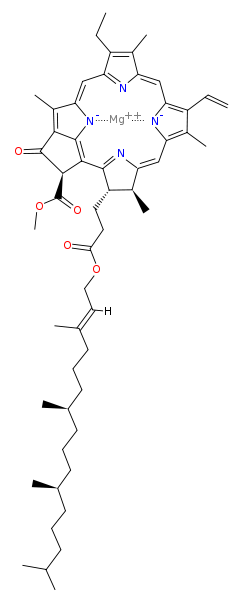
\includegraphics[width=0.5\linewidth]{pictures/hla} \\ a) Хлорофилл A}
\end{minipage}
\hfill
\begin{minipage}[h]{0.49\linewidth}
\center{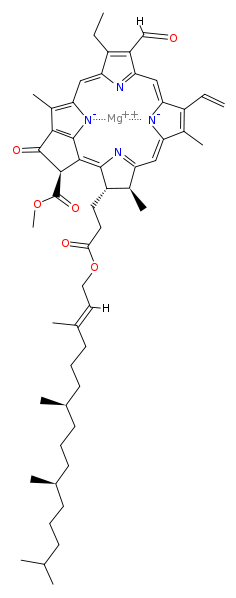
\includegraphics[width=0.5\linewidth]{pictures/hlb} \\ б) Хлорофилл Б}
\end{minipage}
\caption{Схема строения молекулы хлорофилла}

\label{hlorophilus_molecula}
\end{figure}

%%%%%%%%%%%%%%%%%%%%%%%%%%%%%%%%%%%%%%%%%%%%%%%%%%%%%%%%%%%%%%%%%%%%%%%%%%%%%%

%\note{Хлорофилл D дополняет хлорофилл A у некоторых красных и хризофитовых водорослей. Хлорофилл D можно рассматривать как производную от хлорофилла A, в молекуле которого винильная группа при С2 заменена на формильную группу}

\paragraph*{Химические свойства хлорофилла}

\paragraph*{}Ядро хлорофилла обладает гидрофильными свойствами а остаток фитола -- гидрофобными свойствами. Это позволяет молекуле хлорофилла взаимодействовать как с белками, так и с липидами. 

\paragraph*{}Хлорофиллы легкорастворимы в ацетоне, серном эфире, этаноле, метаноле, сероуглероде, бензоле, плохорастворимы в петролейном эфире.

\paragraph*{}При потере магния хлорофилл превращается в \termin{феофитин}, магния и фитола -- в \termin{феофорбид}, только фитола -- в \termin{хлорофиллид}.

\paragraph*{}Рассмотрению химических свойств хлорофилла будет посвящена одна из \hyperlink{chem_hlorophil}{лабораторных работ}.

\note{Окраска хлорофила настолько интенсивная, что на покраску одного гектара тропического леса понадобилось бы лишь одно ведро хлорофилла}

\paragraph*{}Различные типы хлорофилла отличаются и по длине волны поглощаемого света:

\begin{enumerate}

\item Максимумы поглощения хлорофилов A и B лежат в синей части спектра (полоса Соре) 428,5-430 нм и 452,5-455 нм и в красной части спектра 660-662 нм и 642-649 нм (\ris \ref{hlspectr})
\item Максимумы поглощения хлорофилла C (в 80 \% ацетоне) -- 446 нм и 631 нм. 
\item Максимумы поглощения хлорофила D (в диэтиловом эфире) -- 445 нм и 686 нм.

\end{enumerate}

%%%%%%%%%%%%%%%%%%%%%%%%%%%%%%%%%%%%%%%%%%%%%%%%%%%%%%%%%%%%%%%%%%%%%%%%%%%%%%%%%%%%%%%%%%%%%%%%%%%%%%%%%%% 
\begin{figure}
  \centering
       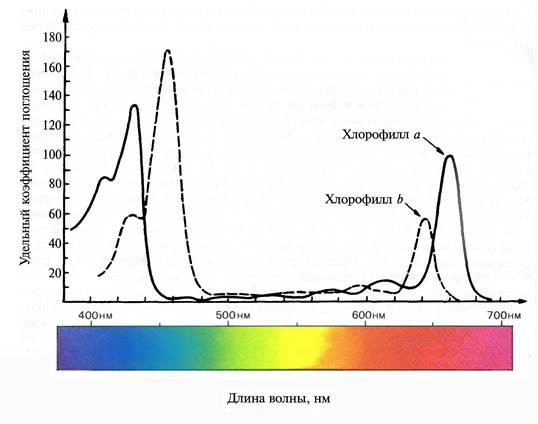
\includegraphics[width=0.6\linewidth]{pictures/hlspectr}
\caption{Спектры поглощения хлорофиллов}
\label{hlspectr}
\end{figure}
%%%%%%%%%%%%%%%%%%%%%%%%%%%%%%%%%%%%%%%%%%%%%%%%%%%%%%%%%%%%%%%%%%%%%%%%%%%%%%%%%%%%%%%%%% 

\paragraph*{}Таким образом, <<полезным>> для фотосинтеза является только свет с определенной длинной волны.

\remember{Та часть солнечного спектра, которая способна возбудить молекулу хлорофилла называется \gls{phtr}}


\note{В физиологических исследованиях важным показателем является отношение вспомогательных хлорофиллов (B, C, D) к хлорофиллу A, которое характеризует степень адаптации к низкому уровню облученности.}

\paragraph*{}Структура молекулы хлорофилла такова, что хлорофилл является хорошим \termin{сенсибилизатором} -- то есть под действием света хлорофилл легко возбуждается и способен вступать в окислительно-восстановительные реакции. Легкость, с которой молекула хлорофилла переходит в возбужденное состояние объясняется системой \hyperlink{question_bounds}{сопряженных} кратных связей в порфириновом кольце.

\subsubsection*{Фотосинтетическая единица}


\paragraph*{}В выделении одной молекулы кислорода в процессе фотосинтеза участвуют не одна, а сразу множество молекул хлорофилла, функционирующие совместно. Эта совокупность молекул получила название \termin{фотосинтетическая единица}. У высших растений в состав \hyperlink{question_photo_unit}{фотосинтетической единицы} обычно входит от 200 до 400 молекул хлорофилла. Таким образом, свет поглощается сотнями молекул хлорофилла, которые затем переносят свою энергию возбуждения к тому месту, где протекают химические реакции. Это место называется \termin{реакционным центром}. 

\paragraph*{}В составе фотосинтетической единицы выделяют два функциональных типа фотосинтетических пигментов:

\begin{itemize}

	\item поглощающие и передающие энергию возбуждения: антенные комплексы
	\item первичные фотохимические реакции: реакционные центры


\end{itemize}

%\paragraph*{}Таким образом, функция большинства молекул хлорофилла в фотосинтетической единице состоит в поглощении света. Только малая доля хлорофиллов, те, которые локализованы в реакционных центрах, участвует в преобразовании света в химическую энергию. 

\note{Хлорофиллы в реакционном центре химически идентичны другим хлорофиллам фотосинтетической единицы, но обладают особыми свойствами, обусловленными их особым окружением. Одно из различий состоит в том, что энергетический уровень возбужденного состояния хлорофиллов реакционного центра ниже, чем у других хлорофиллов, и они поэтому способны улавливать энергию \cite{stier_85}} 

\paragraph*{}Энергия, поглощенная молекулами хлорофилла, перемещается по фотосинтетической единице, пока не достигнет хлорофилла \termin{реакционного центра}. Фотохимическую функцию в составе реакционных центров выполняет хлорофилл A.

\subsubsection*{Реакционные центры}

\paragraph*{}Реакционные центры находятся в центре особых белковых комплексов -- \hypertarget{photosystems}{фотосистем}, интегрированых в мембрану \hyperlink{cell_plastids}{тилакоидов}. 

\paragraph*{}\gls{photosystem} представляет собой функциональную и структурную единицу белковых комплексов, которые осуществляют первичные фотохимические реакции фотосинтеза: поглощение света, преобразование энергии и перенос электронов. 

\paragraph*{}Различают два типа фотосистем -- \gls{fs1} и \gls{fs2}. В \hyperlink{cell_plastids}{хлоропластах} растений присутствуют и \hyperlink{photocooperation}{согласованно} работают оба этих типа фотосистем.

%Первичный акцептор электрона – убихинон в окисленном состоянии тушит флюоресценцию хлорофилла а в составе светособирающего комплекса ФС2. 

\paragraph*{}Реакционным центром \gls{fs1} является длинноволновая форма хлорофилла а с максимумом поглощения при 700 нм ($P_{700}$). 

\paragraph*{}Антенный комплекс \gls{fs2} состоит из 36 молекул хлорофилла A, комплекс \gls{fs1} -- из 96 молекул. Размеры светособирающего комплекса не постоянны и зависят от условий, в которых формируется и функционирует фотосинтетический аппарат.

\remember{Результатом работы реакционных центров является разделение зарядов (отрицательный заряд на внутренней поверхности, мембраны  положительный -- на внешней).} 

\subsubsection*{Электрон-транспортная цепь фотосинтеза}

\paragraph*{}Компоненты \hypertarget{photoetl}{фотосинтетической цепи} переноса электронов локализованы в мембране \hyperlink{cell_plastids}{тилакоидов} (\ris \ref{etl})

%%%%%%%%%%%%%%%%%%%%%%%%%%%%%%%%%%%%%%%%%%%%%%%%%%%%%%%%%%%%%%%%%%%%%%%%%%%%%%%%%%%%%%%%%%%%%%%%%%%%%%%%%%% 
\begin{figure}
  \centering
       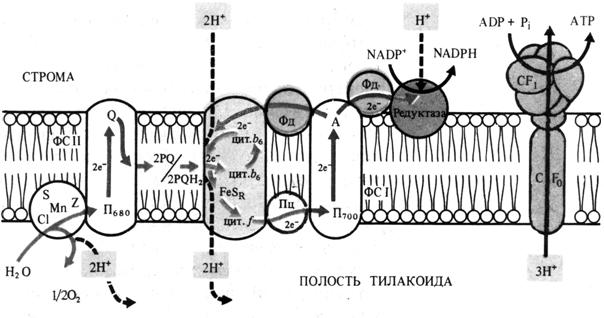
\includegraphics[width=0.8\linewidth]{pictures/etl}
\caption{Схема расположения белков электрон-транспортной цепи на мембране}
\label{etl}
\end{figure}
%%%%%%%%%%%%%%%%%%%%%%%%%%%%%%%%%%%%%%%%%%%%%%%%%%%%%%%%%%%%%%%%%%%%%%%%%%%%%%%%%%%%%%%%%% 

\paragraph*{}Различают следующие компоненты электрон-транспортной цепи:

\begin{enumerate}
	\item Цитохромный комплекс белков-переносчиков электронов, в который входят 2 \gls{cytochrom}а $b_{6}$, \gls{cytochrom} f и железосерный белок Риске FeSR.
	\item Белок ферродоксин, который находится поверхности мембраны со стороны стромы
	\item \hyperlink{enzimes}{Фермент} ФАД-редуктаза, белок пластоцианин, который расположен со стороны просвета \hyperlink{cell_plastids}{тилакоида}.
\end{enumerate}

\paragraph*{}Последовательность переносчиков электронов в \gls{electonykLink} фотосинтеза определяют на основе величины их окислительно-восстановительного потенциала. 

\remember{Электрон самостоятельно может переходить от донора к акцептору, если редокс-потенциал донора (ЕД) меньше, чем редокс-потенциалом акцептора (ЕА). В противном случае перенос электрона происходит в результате фотохимической реакции за счет энергии света.}

\paragraph*{}В цепи транспорта электрона выделяют пять \hyperlink{proteins}{белковых комплексов}, дифференцированных структурно и функционально: 

\paragraph*{}Таким образом, фотосинтетический аппарат растения включает в себя следующие компоненты:

\begin{enumerate}

	\item \gls{fs2}, состоящая из 

		\begin{enumerate}
			\item Хлорофилл $P_{680}$, 
			\item Переносчики электронов -- феофитин, хиноны Q a и $Q_{b}$. 
		\end{enumerate} 

	\item \gls{fs1}, состоящая из 

		\begin{enumerate}
			\item Хлорофилл $P_{700}$, 
			\item переносчики электронов $A_{0}$ (хлорофилл), $A_{1}$ (филлохинон витамин К), 3 железосерных белка FeS
		\end{enumerate}
	
	\item \gls{electonykLink}
\end{enumerate}


\subsection*{Световая фаза фотосинтеза}

\paragraph*{}\termin{\hypertarget{light_stage}{Световая фаза}} -- это этап фотосинтеза, в течение которого за счёт энергии света образуются богатые энергией соединения \gls{atp} и молекулы — носители энергии.

\paragraph*{}Осуществляется на внутренних мембранах \hyperlink{cell_plastids}{хлоропластов}, на которых располагаются молекулы хлорофилла и представляет собой последовательность из фотофизических и фотохимических процессов.

\paragraph*{}В фотофизических реакциях передачи энергии между пигментами и в фотохимических реакциях передачи электронов принимают участие возбужденные молекулы пигментов. У хлорофиллов, фикобилинов и каротиноидов при поглощении кванта света в возбужденное состояние переходят $\pi$-электроны, участвующие в образовании двойной связи.

\subsubsection*{Поглощение света и передача энергии возбуждения}

\paragraph*{}\hyperlink{question_chem_phys}{Преобразование} световой энергии в химическую энергию продуктов фотосинтеза происходит в следующей последовательности.

\begin{enumerate}

\item На первой, \termin{фотофизической} стадии квант света поглощается молекулами хлорофилла и направляется в реакционный центр
\item В реакционном центре происходит следующая стадия -- \termin{фотохимическая}, в результате которой энергия возбужденной молекулы хлорофилла расходуется на разделение зарядов энергия в реакционном центре. 

\remember{Разделение зарядов -- это ключевое событие фотосинтеза, потому что именно на этом этапе происходит преобразование физической формы энергии в химическую \cite{medvedev_2012}}

\item На третьем этапе, в результате \termin{фотохимических} процессов осуществляется синтез \gls{atp} и \gls{nadfh2}, которые являются главными продуктами световой стадии фотосинтеза.

\end{enumerate} 

\paragraph*{}В последующем, энергия, запасенная в продуктах световых реакций используется в темновой (физиологической) фазе фотосинтеза и расходуется на синтез органических соединений и регенерацию акцептора углекислого газа.

\remember{Процесс синтеза \gls{atp} за счет энергии света в процессе световой стадии фотосинтеза называется \hypertarget{photophosforolysis}{фотофосфорилирование}}

\paragraph*{}Различают два пути фотофосфорилирования:

\begin{enumerate}
	\item Циклическое
	\item Нециклическое
\end{enumerate}

\subsubsection*{Циклическое фосфорелирование}

\paragraph*{}Циклическое фотофосфорилирование -- это более простой эволюционно древний путь. В нем участвует \gls{fs1} и цитохромный комплекс и его единственным продуктом является \gls{atp}.

\paragraph*{}При поглощении 2 квантов света хлорофилл $Р_{700}$ переходит в возбужденное состояние и отдает 2 электрона, трем железосерным белкам (FeS). Попав в электрон-транспортную цепь электроны движутся по ее белкам в следующей последовательности: ферридоксину $\rightarrow$ пластохиноны PQ внутри мембраны $\rightarrow$ \gls{cytochrom}ы b6 $\rightarrow$ железосерный белок Риске FeSR $\rightarrow$ пластоцианин. С пластоцианина электрон опять возвращается к молекуле $Р_{700}$. Освобождающаяся энергия используется для синтеза одной молекулы \gls{atp}.

\paragraph*{}Таким образом, электрон движется по кругу -- он выбивается светом из хлорофилла и затем, пройдя по цепи переносчиков возвращается в эту же молекулу.

\subsubsection*{Нециклическое фосфорелирование}

\paragraph*{}При нециклическом фосфорилировании $P_{680}$, поглотив 2 кванта света, переходит в возбужденное состояние и отдает 2 электрона феофитину, затем электроны передает последовательно по следующей цепи из белков хиноны $Q_{a}$ и $Q_{b}$, $\rightarrow$ пластохиноны PQ внутри мембраны $\rightarrow$ железосерный белок FeSR $\rightarrow$ \gls{cytochrom} f $\rightarrow$ пластоцианин и $Р_{700}$ (\ris \ref{acyclfosph}).

\paragraph*{}Молекула хлорофилла $P_{700}$, поглотив 2 кванта света, переходит в возбужденное состояние и отдает 2 электрона, трем железосерным белкам (FeS) $\rightarrow$ ферридоксину $\rightarrow$ ферменту ФАД-редуктазе, которая восстанавливает \gls{nadfh2}. 

\paragraph*{}Недостающие электроны в $P_{700}$ переходят с пластоцианина.

\paragraph*{}Энергия, освобождающаяся при движении электронов от $P_{680}$ (Е=-0,8В)
до $P_{700}$ (Е=+0,4В) используется для синтеза 3 \gls{atp}.

\paragraph*{}Таким образом, при нециклическом фосфорилировании обе фотосистемы \hypertarget{photocooperation}{работают} \hyperlink{question_photocooperation}{согласованно}.

%%%%%%%%%%%%%%%%%%%%%%%%%%%%%%%%%%%%%%%%%%%%%%%%%%%%%%%%%%%%%%%%%%%%%%%%%%%%%%%%%%%%%%%%%%%%%%%%%%%%%%%%%%% 
\begin{figure}
  \centering
       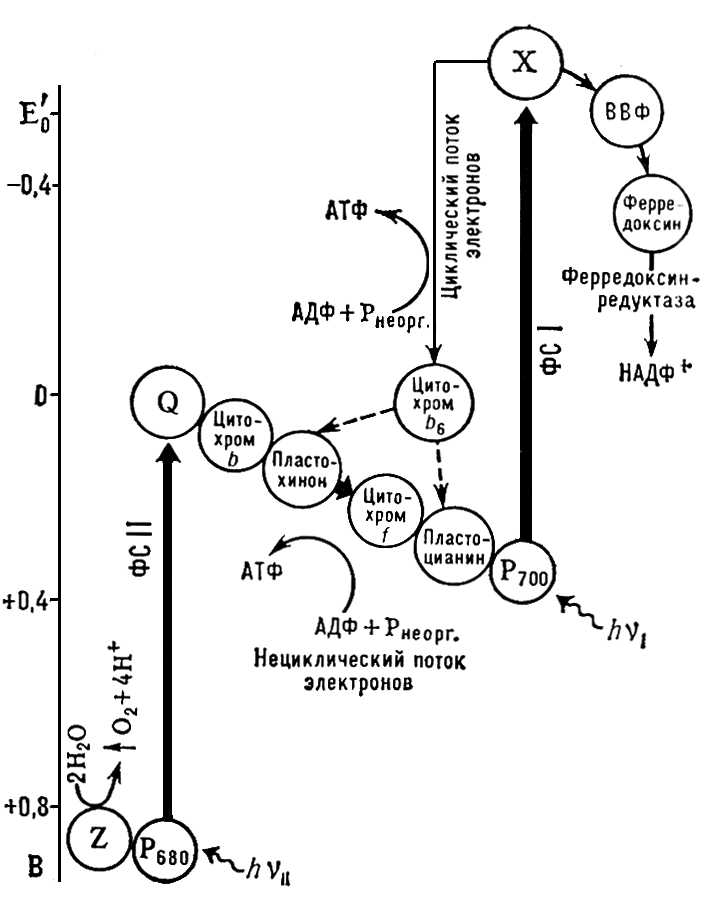
\includegraphics[width=0.4\linewidth]{pictures/acyclfosph}
\caption{Схема ациклического пути фотосинтеза}
\label{acyclfosph}
\end{figure}
%%%%%%%%%%%%%%%%%%%%%%%%%%%%%%%%%%%%%%%%%%%%%%%%%%%%%%%%%%%%%%%%%%%%%%%%%%%%%%%%%%%%%%%%%% 



%\subsubsection*{Совместное функционирование двух фотосистем}

%\paragraph*{}Перенос электронов против термодинамического градиента от воды к НАДФ+ ($\delta E \approx 1,15$ В) происходит за счет энергии двух квантов света с участием двух фотосистем, работающих последовательно. 
%Красное падение (Первый эффект Эмирсона). Квантовый выход снижается в спектральной области, которую поглощают каротиноиды, а также в области длин волн больше 685 нм, в которой интенсивно поглощается хлорофилл а, но не поглощается хлорофилл в. 
%Эффект усиления (Второй эффект Эмирсона). Эффект <<красного падения>> может быть снят при добавочном освещении более коротковолновым светом, поглощаемым хлорофиллом b или каротиноидами.  

\note{Процесс фотофосфорилирования продолжается даже при отрицательных температурах}

\subsubsection*{Фотоокисление воды}

\note{Как было сказано выше, в ходе нециклического фосфорилирования молекула хлорофилла $Р_{700}$ теряет свой, поэтому клетке растения необходим источник электронов, с помощью которого хлорофилл $Р_{700}$ мог бы восполнять потерянные электроны. Таким источником является фотолиз или фотоокисление воды.}

\paragraph*{}Комплекс \hypertarget{photolisys}{фотоокисления} воды интегрирован в белок в составе \gls{fs2}. Реакции фотоокисления воды протекают на внутренней стороне мембран тилакоида. 

\paragraph*{}В общем виде реакция фотоокисления воды идет по следующей схеме:

\paragraph*{}$2H_{2}O \xrightarrow{\text{4 кванта света}} 4H^{+} + 4e + O_{2}$.

\paragraph*{}Таким образом, после удаления четырех электронов из воды образуется молекулярный кислород. Состав каталитического центра, участвующего в фотоокислении $Mn_{4}O_{4}Ca$. В качестве кофактора реакции фотоокисления воды выступают ионы хлора. 

\remember{Именно фотоокисление воды является источником молекулярного кислорода, выделяемого растениями}

\subsubsection*{Стехиометрия сопряжения электронного транспорта и образования АТФ}

\paragraph*{}Фосфорилирование представляет собой процесс синтеза молекулы АТФ из пирофосфата и АДФ за счет свободной энергии, освобождающейся в ходе сопряженной химической реакции, или за счет электрохимического потенциала ионов водорода. 

\note{Поскольку накопление электрохимического градиента в тилакоидах происходит за счет энергии света, синтез \gls{atp} в хлоропластах получил название фотосинтетического фосфорилирования, или фотофосфорилирования.}

\paragraph*{}Реакция синтеза \gls{atp}, катализируемая локализованной в мембране обратимой АТФазой, 
%АДФ + Фн + 3Н+внутр = АТФ + Н2О + 3Н+внешн.

\paragraph*{}Энергетически зависимая стадия синтеза \gls{atp} представляет собой отщепление образованной \gls{atp} от энзимного комплекса.

\note{Образование \gls{atp} в хлоропластах можно вызвать в темноте за счет искусственного создания протонного градиента в условиях кислот-основного перехода. В единицах рН величина градиента ионов водорода, необходимая для синтеза \gls{atp}, составляет 3-3,5 ед. При этом рН стромы составляет величину порядка 7,8-8,0, рН внутри тилакоида -- 4,0-4,5 ед.}
%Электрохимический градиент ионов водорода направлен из внутритилакоидного пространства в строму. Концентрационная составляющая электрохимического градиента существенно превалирует над электрической составляющей. Это достигается выходом из тилакоидов ионов калия и магния.

\paragraph*{}Градиент электрохимического потенциала ионов водорода на мембране тилакоида возникает в результате: 

\begin{enumerate}

\item выхода \gls{proton}ов во внутреннее пространство тилакоида при фотоокислении воды, 
\item связывании ионов водорода в пространстве стромы при восстановлении акцептора электронов \gls{nadfh2}, 
\item транспорта \gls{proton}ов посредством подвижного переносчика – пластохинона.

\end{enumerate}


\subsection*{Темновая стадия фотосинтеза}

\paragraph*{}На темновой стадии\footnote{Темновая стадия -- это традиционное название, не совсем точно отражающее суть процесса. Првильнее было бы называть эту стадию светонезависимой. Реакции темновой стадии не нуждаются в энергии света, однако нуждаются в продуктах световой стадии, поэтому эти реакции не могут идти в темноте, когда продукты световой стадии не вырабатываются}, поглощаемый растениями углекислый газ связывается с различными сахарами. Итогом этой реакции является образование пировиноградной кислоты, а затем и глюкозы.

%Природа первичных акцепторов углекислого газа (углекислоты) Акцептором углерода следует считать органическую молекулу, способную ферментативным путем присоединить молекулу углекислого газа (СО2) или остаток угольной кислоты (НСО3-1, СО3-2). 
\paragraph*{}Процесс присоединения молекулы $CO_{2}$ к органическому соединению с образованием карбоксильной группы называют \termin{карбоксилированием}, а \hyperlink{enzimes}{ферменты}, осуществляющие этот процесс, -- \termin{карбоксилазами}. 

\paragraph*{}Карбоксилирование свойственно как гетеротрофным, так и автотрофным организмам. 

\paragraph*{}Источником энергии для карбоксилирования является \gls{atp}, накопленная во время световой стадии, а источником \gls{proton}ов, необходимых для восстановления углерода из углекислого газа выступают востановленные формы НАДН+Н или \gls{nadfh2} которые так же являются продуктами световой стадии.

\subsubsection*{Фиксация углекислого газа в цикле Кальвина -Бенсона, ключевые ферменты}

%При исследовании фотосинтетического карбоксилирования одновременно решаются вопросы природы первичного акцептора углерода, природы устойчивого первичного продукта и природы фермента. 
\note{Пути фиксации и превращения углерода в процессе фотосинтеза стали понятны благодаря развитию методов хроматографии в сочетании с применением радиоизотопа углерода $^{14}C$. в ходе опытов М. Кальвина, Дж. Бассема, Э. Бенсона}
%Меченый углерод входит в состав карбоксильной группы. Акцептором углекислого газа оказалось пятиуглеродное соединение рибулезо-1,5-бифосфат, а не двухуглеродное, как предполагали вначале. 
%Объектами исследований, которые позволили добиться первых успехов в изучении реакций фотосинтетической фиксации углекислого газа, были зеленые микроводоросли родов Chlorella и Scenedesmus. Успех обеспечили условия проведения экспериментов: включение-выключение света, быстрое снижение концентрации СО 2 от 1 \% до 0,003 \%.
%Группа ученых во главе с М. Кальвином установила, что фотосинтетическая ассимиляция углерода является темновым циклическим ферментативным процессом, в ходе которого расходуется энергия синтезированных во время световой стадии соединений (АТФ и НАДФН+Н), образуются конечные продукты и регенерируется молекула первичного акцептора углерода.
%Позднее выяснилось, что по такому принципу устроены и другие пути фотосинтетического усвоения СО2 или остатка угольной кислоты.
\paragraph*{}Различают три этапа восстановительного пентозофосфатного цикла (ВПФ-цикл) фиксации углерода (\ris \ref{calvin}):

%%%%%%%%%%%%%%%%%%%%%%%%%%%%%%%%%%%%%%%%%%%%%%%%%%%%%%%%%%%%%%%%%%%%%%%%%%%%%%%%%%%%%%%%%%%%%%%%%%%%%%%%%%% 
\begin{figure}
  \centering
       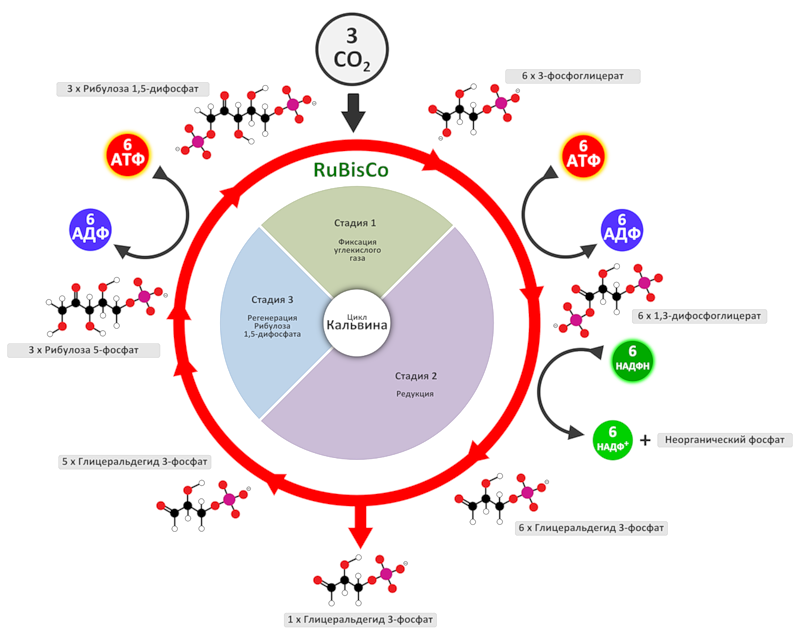
\includegraphics[width=0.6\linewidth]{pictures/calvin}
\caption{Схема ациклического пути фотосинтеза}
\label{calvin}
\end{figure}
%%%%%%%%%%%%%%%%%%%%%%%%%%%%%%%%%%%%%%%%%%%%%%%%%%%%%%%%%%%%%%%%%%%%%%%%%%%%%%%%%%%%%%%%%% 


\begin{enumerate}

\item Карбоксилирование. На этом этапе, молекула $CO_{2}$ соединяется с пятиуглеродным сахаром \termin{рибулозо-1,5-бифосфатом}. В результате образуется две молекул \termin{3-фосфоглицериновой кислоты} (ФГК). Реакцию карбоксилирования катализирует \hyperlink{enzimes}{фермент} \termin{рибулобисфосфаткарбоксилаза} (Сокращенно РуБисКо). \note{Молекулярная масса этого фермента очень высока -- 540 кДа, он состоит из 8 больших (55 кДа) и 8 малых (13 кДа), кодируемых как геномом хлоропластов, так и ядерным геномом. Этот этап фотосинтеза наиболее важен для биосферы. РУБИСКО является наиболее распространенным ферментом в биосфере -- его количество на нашей планете составляет около 10 млн. т, или около 2 кг на каждого жителя Земли. С участием этого фермента фотосинтезирующие организмы Земли ежегодно ассимилируют около 200 млн т $CO_{2}$ , превращая его в органические соединения, используемые всеми живыми организмами планеты \cite{medvedev_2012}}

\item Восстановление 3-\gls{fgac}. На этой стадии \gls{fgac} восстанавливается до 3-фосфоглицеринового альдегида \remember{Путь превращения 3-\gls{fgac} -- это центральное звено темновой стадии }. Этот Процесс идет в два этапа. 

\begin{enumerate}

\item Вначале, под действием фермента фосфоглицераткиназы от молекулы \gls{atp} на 3-\gls{fgac} переносится еще одна фосфатная группа и образуется 1,3-дифосфоглицериновая кислота (1,3-ФГК) с макроэргической связью \cite{medvedev_2012}. 

\item Затем происходит восстановление 1,3-\gls{fgac} в 3-фосфоглицериновый альдегид (3-ФГА) за счет \gls{nadfh2}. Этот процесс катализируется ферментом \termin{триозофосфатдегидрогеназой}. \note{Восстановление 1,3-\gls{fgac} до 3-\gls{fgal} — единственный восстановительный процесс цикла Кальвина, в котором используется \gls{nadfh2}, образуемый в фотохимических реакциях фотосинтеза. Последующие процессы цикла Кальвина необходимы для того, чтобы регенерировать (синтезировать) первичный акцептор $CO_{2}$ — рибулозо-1,5-бисфосфат для того, чтобы он вновь участвовал в фиксации $CO_{2}$.}

\end{enumerate}

\item Регенерация акцептора углекислого газа. На этой стадии, в результате внутримолекулярные перегруппировки фосфорсодержащих сахаров, 5 молекул трехуглеродного соединения \gls{fgal} превращаются в 3 молекулы пятиуглеродно сахара \termin{рибулозо-1,5-бифосфата}. На этом этапе цепь реакций цикла Кальвина замыкается.

\end{enumerate}


%1. Сначала из 3-ФГК с участием фермента фосфоглицераткиназы и АТФ образуется 1,3-дифосфоглицериновая кислота (1,3-ДФГК) с макроэргической связью. 
%2. Далее фермент триозофосфатдегидрогеназа с участием НАДФН+Н восстанавливает 1,3-ДФГК до 3-фосфоглицеринового альдегида (3-ФГА). Таким образом, в реакциях превращения 3-ФГК в 3-ФГА расходуются богатые энергией продукты световой фазы фотосинтеза: 2 молекулы НАДФН+Н и 2 молекулы АТФ.
%3. Дальнейшие реакции ВПФ-цикла направлены на превращение трехуглеродных соединений (3-ФГА и его изомера диоксиацетонфосфата (ДОАФ)) в пятиуглеродный акцептор СО2 – рибулозо-1,5-бисфосфат, а также на получение продуктов фотосинтеза (сахароза, крахмал). 
 

%В реакции превращения рибулозо-5-фосфата в рибулозо-1,5-бисфосфат расходуется еще одна молекула АТФ, образованная в результате фотофосфорилирования.
%Из реакций ВПФ-цикла для дальнейшего превращения в продукты фотосинтеза необходимо вывести молекулу фосфорсодержащего сахара. Такой молекулой с минимальным числом атомов углерода является 3-ФГА (или 3-ФГК). Поэтому для баланса цикла в него необходимо ввести три молекулы СО 2. 
%Тогда при полном обороте цикла из пяти молекул 3-ФГК можно получить в конечном итоге три молекулы рибулозо-1,5-бисфосфата. При этом на осуществление реакций требуется 6 молекул НАДФН+Н (если из цикла уходит 3-ФГА) и 9 молекул АТФ. Соотношение НАДФН+Н/АТФ, равное 2/3, должно обеспечивать световые реакции фотосинтеза.

\paragraph{Баланс веществ в цикле Кальвина}

\paragraph*{}Таки образом, в ходе реакций цикла Кальвина синтезируется шесть молекул \gls{fgal}, одна из которых выводится из цикла, а пять идут на регенерацию рибулезо-2-фосфата.  

\paragraph*{}Так как на синтез глюкозы необходимы 2 молекулы \gls{fgal}, образующиеся в результате двух оборотов цикла Кальвина, можно подсчитать, что на синтез одной молекулы глюкозы расходуется 12 молекул \gls{nadfh2} и 18 молекул \gls{atp}.

\subsubsection*{Фиксация углекислого газа в цикле Хэтча-Слэка-Карпилова}

\note{Основой для биохимических исследований фотосинтеза у С4-растений стали работы Коршака и его сотрудников (Гонолулу), в СССР – Ю.С. Карпилова и его сотрудников, в Австралии – Хэтча, Слэка и Джонсона.}

\paragraph*{}Растения, способные усваивать углекислый газ по C4 пути имеют некоторые характерные черты анатомического строения:

\begin{enumerate}
	\item Проводящие пучки листьев таких растений окружены двойным слоем зеленой ассимиляционной паренхимы, внешний слой которой состоит из клеток мезофилла, а внутренний из клеток обкладки пучка. 
	\item При этом клетки обкладки отличаются как структурно так и функционально:
	\begin{enumerate}
	
		\item \hyperlink{cell_plastids}{Хлоропласты} клеток обкладки содержат много зерен крахмала и не содержат гранн
		\item В хлоропластах клеток обкладки наблюдается низкая активность фотосистемы 2, в результате чего практически не происходит \hyperlink{photolisys}{фотолиза} воды и не выделяется кислород.
	
	\end{enumerate}	 
		
	\item В листе содержится много воздушных полостей
	
\end{enumerate}

\paragraph*{}Так же как и в случае цикла Кальвина, при образовании С4-соединений в цикле Хэтча-Слэка-Карпилова, расходуются продукты \hyperlink{light_stage}{световой фазы} фотосинтеза (\gls{atp} и \gls{nadfh2}), однако, C4-путь фиксации углерода заметно отличается от цикла Кальвина. Можно выделить следующие черты, отличающие С4-растения от С3-растений следующие: 

\begin{enumerate}

	\item Источником $CO_{2}$ для ВПФ-цикла служат С4-органические кислоты, а не $CO_{2}$ атмосферы; 
	\item Первоначально атмосферный углекислый газ соединяется с С3-соединением \gls{fep}, которое превращается в С4-соединение щавелево-уксусной кислоты (оксалоацетат), или ЩУК, с участием цитоплазматического фермента \gls{fep} – карбоксилазы; 
	\item У C4 растений реакции фиксации $CO_{2}$ пространственно разделены между двумя типами клеток. 
	\item При этом С4-соединения выполняют роль челноков, переносящих углерод и свободную энергию в клетки обкладки проводящих пучков, где локализованы ферменты ВПФ-цикла; 
	\item После декарбоксилирования образующиеся С3-соединения возвращаются в клетки, где локализованы соответствующие им карбоксилазы. 
	%\item Вторичное включение $CO_{2}$ в ВПФ-цикл с образованием сахарозы (клетки обкладки проводящих пучков).

\end{enumerate}


\note{В настоящее время составляет около 10000 видов однодольных и двудольных растений, среди которых такие сельскохозяйственно-значимые культуры как кукуруза, сорго, просо и сахарный тростник}

\paragraph*{}Появление C4-пути связано с тем, что \hyperlink{enzimes}{фермент} РуБисКо обладает высокой окислительной активностью, так как изначально был приспособлен для работы в условиях высокой концентрации углекислого газа. По этой причине работа этого фермента в условиях низкой концентрации углекислого газа малоэффективна. Карбоксилазы С3-соединений, в отличие от фермента Рубиско, не имеют оксигеназной активности и способны работать при крайне низких отношениях $CO_{2}/O_{2}$ в атмосфере. Таким образом, С4-путь позволяет увеличить эффективность как первичной фиксации углекислого газа, так и вторичной, связанной с ферментом Рубиско (за счет увеличения концентрации $CO_{2}$ и снижения концентрации $O_{2}$).

\paragraph*{}Дефицит углекислого газа может наблюдаться в условиях засушливого климата, когда устьица подолгу закрыты и, следовательно, поступление углекислого газа из атмосферы к ассимиляционному мезофиллу затруднено.

\remember{C4-путь ассимиляции углерода это приспособление к существованию растений в условиях низкой концентрации углекислого газа. Смысл C4-пути состоит в том, что углекислый газ изначально концентрируется в виде четырехуглеродных сахаров в клетках обкладки, а затем переправляется в клетки мезофилла. За счет этого в клетках мезофилла создается нужная для работы РуБисКо концентрация углекислого газа}

\subsubsection*{Первичные продукты фотосинтеза}

Первичными можно считать продукты фотосинтеза, образующиеся из промежуточных соединений ВПФ-цикла раньше конечных углеводов. 
К таким продуктам у хлореллы относятся аминокислоты 

\begin{enumerate}

\item аланин, 
\item серин, 
\item аспарагиновая кислота, 
\item глутаминовая кислота. 

\end{enumerate}

\paragraph*{}Аминокислоты, появившиеся в хлоропластах во время фотосинтеза, включаются в белок раньше и с большей эффективностью, чем аминокислоты, образованные в темновых реакциях превращения сахаров. 
На свету активируется синтез липидов, в который вовлекаются ДОАФ и двухуглеродные фрагменты, присутствующие в реакциях с участием транскетолаз.

\paragraph*{}Факторами, регулирующими пути усвоения $CO_{2}$ при фотосинтезе, являются 

\begin{enumerate}

\item физиологическое состояние растения, 
\item освещенность, 
\item водоснабжение,
\item минеральное питание, 
\item содержание $CO_{2}$. 
\item Отношение восстановленного \gls{nadfh2} к \gls{atp}. При недостатке \gls{atp} превращение 3-\gls{fgac} в 3-\gls{fgal} может быть затруднено и 3-\gls{fgac}будет направлена на образование \gls{fep}.

\end{enumerate}

\subsection*{Фотодыхание}

\paragraph*{}Фотодыхание – процесс поглощения кислорода и выделения $CO_{2}$ хлоропластами на свету. Точно измерить интенсивность фотодыхания трудно, так как при этом одновременно идут и фотосинтез и митохондриальное дыхание. 

\paragraph*{}Разветвление процессов фотосинтеза и фотодыхания происходит на уровне ключевого фермента ВПФ-цикл-Рубиско. Фермент проявляет свойства оксигеназы. Конечным продуктом фотодыхания, как и ВПФ-цикла, является молекула \gls{fgac}. Поэтому фотодыхание можно рассматривать как биохимический шунт, обеспечивающий работу цикла в условиях, когда фермент Рубиско функционирует при недостатке $CO_{2}$ или избытке кислорода.

\paragraph*{}В основе фотодыхания лежит гликолатный путь С3-растений. При этом, процесс фотодыхания имеет следующие особенности: 

\begin{enumerate}
	\item $CO_{2}$ образуется в реакции превращения двух молекул глицина в серин
	\item кислород расходуется как при образовании гликолата с участием фермента Рубиско, так и при окислении гликолата с участием гликолатоксидазы
	\item образуется свободный аммиак
	\item в гликолатном цикле расходуется энергия \gls{atp} и \gls{nadfh2}
	\item \gls{fgac} может расходоваться на синтез сахарозы и крахмала (гликогенолиз)
	\item Цикл основан на челночном переносе метаболитов между компартметами клетки – цитоплазмой, хлоропластами, митохондриями и пероксисомами
	
\end{enumerate}

\paragraph*{}Фотодыхание свойственно С3-растениям и эукариотическим водорослям.

\subsection*{Вопросы и задания для самоконтроля}

\begin{enumerate}
	\item По учебнику органической химии повторите суть реакции \hypertarget{eterefication}{этерефикеции}. Для каких классов химических веществ характерна эта реакция?

	\item Что такое \hyperlink{question_photo_unit}{фотосинтетическая единица}, фотосистема, реакционный центр?

	\item Какие особенности \hypertarget{question_bounds}{структуры} молекулы хлорофилла позволяют ей легко возбуждаться под действием солнечного света?

	\item Какие процессы световой стадии фотосинтеза являются \hypertarget{question_chem_phys}{фотофизическими}, а какие -- фотохимическими и почему?

	\item Объясните, в чем заключается \hypertarget{question_photocooperation}{согласованная} работа двух фотосистем при нециклическом фосфорилировании?
\end{enumerate}